\section{Historical and external controls}
\label{sec:extended-operating}
The operating analysis uses the 704 historical candidates in Section~\ref{sec:evidence}. The external controls below use the original boosted-tree nominations on the 216 fixed candidates in Section~\ref{sec:transport}.

\paragraph{Operating the veto.}
On search paths, the minimum vote vetoed 184 of 189 breaches (97.4\%) and 194 of 211 passes (91.9\%). Compared with voting only on the empty and full restorations, the interiors caught 11 additional breaches and vetoed 20 additional passes. The paired changes in true- and false-positive rates were $+5.82$ percentage points (95\% interval $[0,13.56]$) and $+9.48$ ($[4.57,15.14]$). On drawn deletions, the minimum vote caught 161 of 163 breaches and vetoed 178 of 216 passes. The interiors added zero detections ($[0,0]$ points) and nine false alarms ($+4.17$ points, $[0.46,9.14]$). The intervals resample tasks and folds, retaining proposals, outcomes and decisions together (30,000 paired draws). They condition on the fitted models and test folds. Seven of the eleven additional detections came from Sonar. With unit false-alarm cost, the interiors repay their 20 extra path false alarms only when a missed breach costs more than $20/11$. On the pooled paths a cutoff at one quarter of the anchor or a constant veto had lower cost than the separating vote at every miss price. Appendix~\ref{sec:refit} gives the full rates, cost curves and learner sensitivities.

\paragraph{What transfers to another task?}
A deletion fraction alone ties all proposals at a given width. We therefore fitted ridge logistic models predicting a refit breach from (i) the deletion fraction with fixed spline terms, (ii) those terms plus the removed share of split gain and rank mass, and (iii) these features plus continuous losses on the empty and full restorations. We compared (iii) with an otherwise identical model adding the largest dissent fraction in any restoration. Each model was trained without any observations from the task where it was evaluated. Scaling and the ridge penalty were identical across models. Tasks received equal weight, as did folds within a task and proposals within a fold. These analyses are retrospective because the collection's outcomes were already known when the comparisons were specified.

\begin{table}[tb]
\centering
\caption{Adding the worst dissent fraction to a predictor using width, Gain and continuous endpoint losses. Lower binary log loss indicates better breach probabilities. Paired 95\% intervals resample the 14 tasks with their out-of-task predictions fixed. The collections share 75 proposals.}
\label{tab:strong-risk}
\small
\begin{tabular}{llrrr}
\toprule
Train on other tasks & Test proposals & Endpoints & With dissent & Paired difference [95\% interval]\\
\midrule
Path & Path & .5742 & .5798 & $+.0056\ [-.0120,.0321]$\\
Path & Drawn & .5758 & .5585 & $-.0173\ [-.0284,-.0056]$\\
Drawn & Path & .5808 & .5793 & $-.0016\ [-.0199,.0191]$\\
Drawn & Drawn & .5407 & .5228 & $-.0179\ [-.0373,.0020]$\\
Unique union & Unique union & .5471 & .5391 & $-.0079\ [-.0216,.0073]$\\
\bottomrule
\end{tabular}
\end{table}

The clearest change occurred when a model trained on paths scored drawn proposals on the omitted task (Table~\ref{tab:strong-risk}). Restricting the target to the same retained width and the observed range of deleted gain mass on the source fold retained 116 of 379 drawn proposals. The paired change was $-.0232$ there ($[-.0422,-.0051]$), and $-.0137$ ($[-.0399,.0138]$) on the 41 remaining after excluding shared supports. The restriction changes the population, and its interval widens as coverage decreases. For the unique union, adding Gain to width alone reduced log loss by .0276 ($[.0088,.0436]$ improvement). Adding dissent to the richer endpoint baseline yielded a smaller, less precise gain. These are conditional prediction comparisons under different proposal distributions. They do not isolate a causal effect of the search path.

\paragraph{Historical opportunity.}
On the 14 PMLB tasks, 41 folds could support a separate guard, including one with a singleton anchor. The minimum vote tied at zero on all candidates in 32 of 40 actionable folds. Against a Gain prefix, it increased mean $U$ from 9.33\% to 10.12\%, entirely on one New Thyroid fold. Breaches rose from one to three. Subsequent refits of every candidate showed that on 18 of 40 folds no candidate met the outer tolerance. On two more the guard excluded every outer pass. On the remaining 20 at least one candidate passed both checks. The corresponding task-weighted ceilings were 24.90\% for outer passage alone and 22.57\% for joint passage, compared with 45.91\% nominal savings if every proposed width were acceptable. This retrospectively scored pool motivated a test that retains the magnitude of the masked losses.

\paragraph{Ten tasks fixed before scoring.}
We selected ten previously unused UCI classification tasks with numeric or ordinal inputs, 4--41 predictors and 210--17,898 records. The list, policies, contrasts and primary tolerance were specified locally before evaluating the tasks. We used all three stratified outer folds per task. Within each development split we assigned 75\% of records to fitting, and split the remainder equally into proposal and guard samples. Imputation used only the corresponding training partition. We recorded selections and outer predictions for all 30 folds before running the outer scorer. The low-fidelity rule and the plan to refit every candidate were separately fixed before inspecting the predictive results. Table~\ref{tab:transport-tasks} identifies each source and gives its paired outcomes.

\begin{table}[tb]
\centering
\caption{Outcome of nominating one candidate for a full XGBoost refit. $U$ is the percentage of anchor columns saved when the final fit meets every tolerance. Breach rates and distinct nomination masks are means over tasks, weighting folds within task equally. Both uniform rows give exact expected returns followed by the same guard. The top-vote lottery draws only among maximizers. Its nomination masks were not separately timed.}
\label{tab:transport}
\small\setlength{\tabcolsep}{5.0pt}
\begin{tabular}{@{}lrrr@{\quad}rrr@{}}
\toprule
 & \multicolumn{3}{c}{10 tasks, 30 folds} & \multicolumn{3}{c}{6 wider tasks, 16 folds}\\
Nomination & $U$ (\%) & Breach (\%) & Masks & $U$ (\%) & Breach (\%) & Masks\\
\midrule
Uniform, whole pool & 5.49 & 8.89 & 0 & 7.07 & 12.96 & 0\\
Gain prefix & 0.00 & 13.33 & 0 & 7.34 & 16.67 & 0\\
Minimum vote & 1.33 & 13.33 & 5.90 & 7.34 & 16.67 & 14.89\\
Vote with uniform tie-break & 6.16 & 8.47 & --- & 9.49 & 13.89 & ---\\
Vote with point tie-break & 7.29 & 6.67 & 5.80 & 7.34 & 16.67 & 14.78\\
All-context margin & 7.29 & 13.33 & 25.33 & 7.34 & 16.67 & 85.11\\
Point margin & 7.29 & 6.67 & 4.20 & 7.34 & 16.67 & 7.94\\
Eight-round refits & 6.33 & 13.33 & 0 & 10.13 & 16.67 & 0\\
\midrule
Attainable $U$ with guard & 13.51 & & & 21.05 & & \\
\bottomrule
\end{tabular}
\end{table}

The primary vote-minus-Gain difference in $U$ was $+1.33$ percentage points (paired task bootstrap 95\% interval $[0,4.00]$). The minimum vote changed two nominees and one final support. Its sole gain came from Seeds. On 16 of 20 actionable folds every nominee had zero worst-context approvals. The primary all-context-margin contrast against Gain was $+7.29$ points ($[1.52,14.45]$), with gains on five folds across four tasks. The all-context margin changed 12 nominations and eight final supports relative to Gain. Omitting the two related crop datasets, Dry Bean and Rice, reduced this gain to 4.95 points. Intervals describe 30,000 paired resamples of these ten tasks, separately for each contrast. All ten nominations on which the all-context margin and vote differed had tied at zero under the vote. For example, on the first Dry Bean fold both five-column nominees passed the guard. The Gain prefix, also chosen by the vote, gave 88.34\% outer accuracy against 91.34\% for the anchor. Changing one column, as both margin rules did, gave 91.27\%. The continuous score broke a tie that changed whether the deletion met tolerance.

The point margin obtained the same $U$ as the full margin on every fold. Their nominees differed six times. In two instances, on Seeds and Steel, the full margin admitted a deletion the point rule avoided, and both breached the outer tolerance. The original exhaustive implementation of the full margin averaged 25.3 distinct nomination masks per fold versus 4.2 for the point margin. The eight-round control used 4.2 extra fits per fold, taking an average of 0.051 seconds for that screening stage. Its $U$ difference from the point rule was $-0.96$ points ($[-5.66,3.89]$). All policies used the same full-fidelity budget of one initial and one final fit on every fold plus an anchor and candidate guard fit on each actionable fold. Whole-pipeline timing and nomination counts answer different cost questions.

\paragraph{Which deletions could have worked?}
We recorded genuine guard and outer fits for all 106 non-anchor candidates on the 20 actionable folds. Of 34 candidates meeting outer tolerance, 27 also passed the guard. Fifteen other candidates passed the guard and breached outside it. On ten of the actionable folds there was no outer pass, on one the guard excluded every outer pass, and on nine a candidate passed both checks. Accounting for the ten singleton anchors gives 29.07\% nominal savings, 15.18\% attainable using the outer results alone and 13.51\% when the guard also has to accept. These are hindsight ceilings on the sampled candidates. The point rule realized five of the nine available fold opportunities.


\paragraph{A second panel with wider inputs.}
We next froze an independent six-source comparison before scoring its 16 planned splits. The sources contain 72--856 features. CNAE-9 and Semeion use row-level folds, Parkinson uses participant-level averages of three recordings, Ozone and SECOM use expanding chronological windows, and Urban Land Cover uses the released train/test split from one aerial image (Appendix~\ref{sec:wide-details}). We specified the all-context margin versus point as primary. A practically material benefit required a lower 95\% paired task-bootstrap endpoint above five percentage points of $U$ and no increase in mean breach rate. Five points correspond roughly to one additional successful half-width deletion per ten decisions.

Fifteen folds offered a deletion, yielding 110 distinct candidates. Gain, vote, point and all-context margins achieved identical $U$ on all 16 folds, with six admissions and three breaches per policy. Their equal-source mean was 7.34\%. All six task differences were zero, so both the observed bootstrap interval and the leave-one-source-out range for the primary contrast were $[0,0]$. Resampling six ties does not determine equivalence on future sources. The full margin used 1,334 nomination masks across the folds, versus 125 for point, while each arm used 62 full-fidelity fits. Full and point disagreed on two nominees and one final support. On one SECOM fold the full margin improved outer AUC from .6078 to .7706 with unchanged accuracy (.9649). Average precision was .0792 and .1517, respectively, against .1711 for the anchor. Both missed its 5\% allowance. That fold accounts for their entire mean AUC difference of .00905.

\paragraph{How large a difference could the guard leave?}
The final supports constrain a comparison before the test labels are scored. Let $L_f,R_f$ be the supports returned by two policies on fold $f$, with removal fractions $s_{Lf},s_{Rf}$ and nonnegative study weight $w_f$. When the same support produces the same fit, its contribution cancels. On each remaining fold passage multiplies the respective saving by either zero or one. Consequently, for the study-weighted utility difference $\Delta U$,
\begin{equation}
 -\sum_{f:L_f\ne R_f}w_f s_{Rf}\ \leq\ \Delta U\ \leq\
 \sum_{f:L_f\ne R_f}w_f s_{Lf}\,.
 \label{eq:opportunity-bound}
\end{equation}
The bound allows passage bits of distinct supports to vary freely. Shared test labels can restrict which combinations are attainable. The retrospective calculation requires only the sealed returns, training procedure and study weights.

On the wider panel the sole XGBoost disagreement after the guard was on SECOM, where both policies kept 69 of 138 columns and the fold carried weight $1/18$. The all-context-minus-point difference therefore lay between $-2.78$ and $+2.78$ points for \emph{any} outer labels. The five-point primary target had become unattainable before the scorer ran. Moreover, $(5/6)^6$ of empirical six-source bootstrap draws omit SECOM, precluding a positive 95\% lower endpoint even if only its full-margin nominee passed. On the ten-task panel only Seeds and Steel supplied final disagreements. In each case the point rule returned the anchor and the full rule halved it. The interval before scoring was $[0,3.33]$ points. The outer outcomes supplied the additional observation that both extra admissions breached.

\paragraph{Does breaking an integer tie recover the gain?}
After the ten-task results and before scoring the wider panel, we specified a rule that maximizes the original integer vote, using the point margin only to break ties. This preserves every strict ordering by vote. Evaluating candidates in descending point-margin order permits exact pruning as soon as the current worst count cannot beat the incumbent. On the first panel this refinement increased $U$ by 5.96 points over the original vote ($[0,13.33]$) and gave the same predictions as point alone. On the wider panel it again gave the same final outcomes as point. It used 5.80 and 14.78 masks per fold on the respective panels. The clocks for the refinement and original policies came from different runs.

To separate the contribution of the point score from the choice of Gain as a tie-breaker, we retrospectively averaged over all candidates tied for the maximum vote on each fold. This keeps every strict vote preference and applies the same guard. On the first panel a uniform top-vote tie-break saved 6.16\% within tolerance and breached on 8.47\% of folds in expectation. Of the 5.96-point gain from switching Gain to point tie-breaking, 4.82 points were already available by randomizing the ties. The remaining 1.14-point point-minus-random difference had a paired task interval of $[-1.05,3.39]$. On the wider panel the top-vote lottery saved 9.49\% with 13.89\% breaches, and the point tie-break saved 7.34\% with 16.67\% breaches (difference in savings $-2.15$ points, $[-6.45,1.85]$). Only eight of 20 actionable first-panel folds and five of 15 wide-panel folds contained both positive- and zero-utility alternatives among the maximizing candidates.

A crossed comparison of one or four panels with empty or all restorations also gave identical $U$ across all four continuous policies on both panels at the primary tolerance. In the first panel, adding the three reweightings at the empty restoration kept two outer breaches. Adding interior restorations on one panel gave three, and combining interiors with four panels gave four. Their equal $U$ masks these differences.

\paragraph{What does the score buy over a lottery?}
Because every candidate was refitted, the expected $U$ of a uniform nomination followed by the same guard can be computed without simulation. On a fold with $M$ candidates of common width, it equals the removal fraction times the number passing both tests divided by $M$. It is zero at a singleton anchor. On the first panel the point rule gained 1.80 points of $U$ over this baseline ($[-0.70,4.31]$), with a breach-rate difference of $-2.22$ points ($[-8.06,3.06]$). On the wider panel the corresponding differences were $+0.27$ points ($[-6.45,8.89]$) and $+3.70$ breach points ($[-4.63,14.58]$). Figure~\ref{fig:opportunity} shows the task-level opportunities. The eight-round control achieved $U=10.13\%$ on the wider panel, 3.06 points above the lottery ($[0.56,5.89]$), with the same mean breach rate as the point rule and an additional small fit for the anchor and each eligible candidate.

\begin{figure}[tb]
\centering
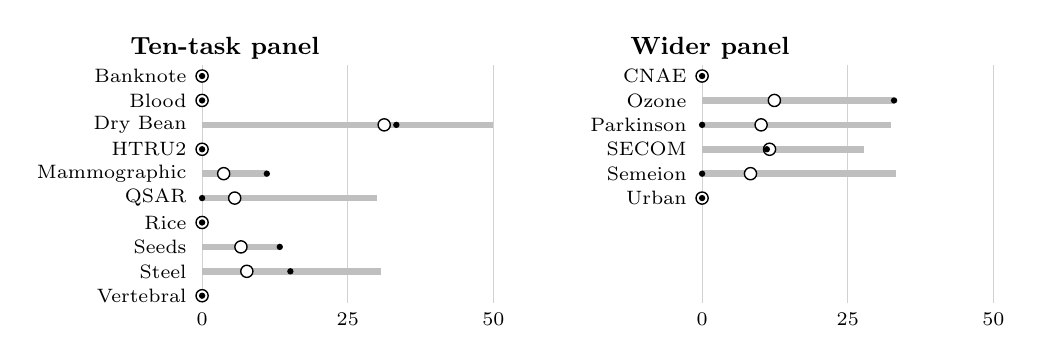
\begin{tikzpicture}[x=.074cm,y=.31cm,font=\scriptsize]
\foreach \offset/\heading in {0/{Ten-task panel},6.35/{Wider panel}}{
\begin{scope}[xshift=\offset cm]
\node[anchor=west,font=\small\bfseries] at (-14,11.15) {\heading};
\foreach \x in {0,25,50}{
 \draw[gray!35,thin] (\x,0.7)--(\x,10.45);
 \node[anchor=north] at (\x,.7) {\x};
}
\end{scope}}
\foreach \y/\name/\point/\lottery/\ceiling in
 {10/Banknote/0/0/0,9/Blood/0/0/0,8/{Dry Bean}/33.333/31.250/50,
  7/HTRU2/0/0/0,6/Mammographic/11.111/3.704/11.111,5/QSAR/0/5.598/29.966,
  4/Rice/0/0/0,3/Seeds/13.333/6.667/13.333,2/Steel/15.152/7.677/30.707,1/Vertebral/0/0/0}{
 \node[anchor=east] at (-1,\y) {\name};
 \draw[line width=2.4pt,gray!50] (0,\y)--(\ceiling,\y);
 \draw[black,fill=white,line width=.5pt] (\lottery,\y) circle[radius=2.2pt];
 \fill[black] (\point,\y) circle[radius=1.15pt];}
\begin{scope}[xshift=6.35cm]
\foreach \y/\name/\point/\lottery/\ceiling in
 {10/CNAE/0/0/0,9/Ozone/32.946/12.403/32.946,8/Parkinson/0/10.127/32.340,
  7/SECOM/11.111/11.574/27.778,6/Semeion/0/8.305/33.221,5/Urban/0/0/0}{
 \node[anchor=east] at (-1,\y) {\name};
 \draw[line width=2.4pt,gray!50] (0,\y)--(\ceiling,\y);
 \draw[black,fill=white,line width=.5pt] (\lottery,\y) circle[radius=2.2pt];
 \fill[black] (\point,\y) circle[radius=1.15pt];}
\end{scope}
\end{tikzpicture}
\caption{Fraction of anchor columns saved within tolerance (percent), averaged over each task's folds. A gray bar ends at the largest attainable mean with the prescribed guard. Open circles mark the exact expected return under uniform nomination and solid dots the point margin. A dot inside a circle indicates matching values. On Parkinson and Semeion some candidate could pass both checks, yet point recovered none of those opportunities.}
\label{fig:opportunity}
\end{figure}


A user may also charge for a breach separately from receiving zero savings. For a charge $h$ in units of a full anchor's value, net return is $U-h\,\mathbf 1\{\mathrm{breach}\}$. At the illustrative price $h=1$, the point rule and the uniform lottery returned $+0.63$ and $-3.40$ points on the first panel (paired difference $+4.03$, $[-1.65,10.72]$). On the wider panel they returned $-9.32$ and $-5.89$ points ($-3.43$, $[-17.26,11.17]$). These pointwise intervals resample whole tasks and condition on the measured candidate outcomes. The five-point primary decision criterion concerned $U$ itself.



\paragraph{Keeping the nominees and changing the learner.}
The preceding comparisons use boosted trees for nomination, guard and final fit. After inspecting their outcomes, we fixed a second learner and all analysis settings before scoring its results. Each original tree-derived candidate and anchor was refitted by standardized L2 logistic regression. Each guard decision and outer evaluation used the logistic anchor trained on the same rows as the candidate. On the ten-task panel the point and all-context rules again gave equal mean $U$ (5.78\%), with one and two breaches, respectively. The guarded uniform choice gave 6.05\%.

On the wider panel vote and point had tied under boosted-tree refits. Under logistic refits their mean savings differed. The vote gave 19.16\% mean $U$, point gave 8.21\%, and the Gain prefix gave 16.55\%. This exploratory vote--point contrast was added after seeing the receiver results. The difference of 10.95 points came from Parkinson and Urban (paired task interval $[0,27.61]$). Urban contributes one entire source weight through a single official split. Relative to Gain, the vote gained 2.61 points ($[0,7.84]$), entirely on Parkinson, and incurred two breaches across 16 folds versus three for Gain and point. The all-context margin reached 10.83\%, gaining 2.61 points over point on Parkinson alone, with unchanged breach rate. Relative to uniform nomination, the full margin changed $U$ by $-0.27$ points ($[-2.58,1.44]$) on the first panel and $-0.16$ ($[-11.14,10.26]$) on the wider panel. The logistic guard alone bounded the full-minus-point contrast at $[0,1.67]$ points on the ten tasks and $[0,2.61]$ on the wider tasks. The wider result attained this upper endpoint. Table~\ref{tab:receiver} gives the matched comparisons. Comparisons within a learner use its own refitted anchor. The absolute values of $U$ for the two learners can therefore differ even for the same nominee.

The expected uniform return averages over nominations. For a single run, independently drawing one nominee per fold can match a deterministic policy by chance. We computed the exact distribution of the task-weighted mean by convolving the fold-specific probabilities of joint guard and outer passage at the observed widths. With the XGBoost fits, the probability of matching or exceeding the point rule's $U$ was 22.06\% on the ten-task panel and 50.18\% on the wider panel. With logistic refits on the wider panel, the corresponding probability for the minimum vote was 8.34\%. These probabilities condition on these precise pools, fitted models, outcomes and fold weights. Only the random nominations vary.


\paragraph{Sensitivity to the masking values.}
On the same 216 candidates we retrospectively replaced each hidden coordinate block with values copied jointly from a fitting row, averaging the predicted class probabilities over 16 donors before computing metrics~\cite{covert2020sage,covert2021removing}. Two fixed donor draws gave opposite all-context-minus-point results for wide-panel XGBoost refits, $+5.44$ points on the first draw and $-5.50$ on the second. Corresponding logistic differences were $+5.28$ and zero. These are nomination outcomes for two finite approximations to marginal integration. Appendix~\ref{sec:masking-background} gives the draw-specific results.
